% scikeds Extract German (Template)
%
% (c) Karsten Reincke, Frankfurt a.M. 2012, ff.
%
% This text is licensed under the Creative Commons Attribution 3.0 Germany
% License (http://creativecommons.org/licenses/by/3.0/de/): Feel free to share
% (to copy, distribute and transmit) or to remix (to adapt) it, if you respect
% how you must attribute the work in the manner specified by the author(s):
% \newline
% In an internet based reuse please link the reused parts to scikeds.fodina.de
% and mention the original author Karsten Reincke in a suitable manner. In a
% paper-like reuse please insert a short hint to scikeds.fodina.de and to the
% original author, Karsten Reincke, into your preface. For normal quotations
% please use the scientific standard to cite
%
% select the document class
% S.26: [ 10pt|11pt|12pt onecolumn|twocolumn oneside|twoside notitlepage|titlepage final|draft
%         leqno fleqn openbib a4paper|a5paper|b5paper|letterpaper|legalpaper|executivepaper openrigth ]
% S.25: { article|report|book|letter ... }
%
% oder koma-skript S.10 + 16
\documentclass[
  DIV=calc,
  BCOR=5mm,
  11pt,
  headings=small,
  oneside,
  abstract=true,
  toc=bib,
  english,ngerman]{scrartcl}
  
%%% (1) general configurations %%%
\usepackage[utf8]{inputenc}

%%% (2) language specific configurations %%%
\usepackage[]{a4,babel}
\selectlanguage{ngerman}

% package for improving the grey value and the line feed handling
\usepackage{microtype}

%language specific quoting signs
\usepackage{csquotes}



%%% (3) layout page configuration %%%

% select the visible parts of a page
% S.31: { plain|empty|headings|myheadings }
%\pagestyle{myheadings}
%\pagestyle{headings}

% select the wished style of page-numbering
% S.32: { arabic,roman,Roman,alph,Alph }
\pagenumbering{arabic}
\setcounter{page}{1}

% select the wished distances using the general setlength order:
% S.34 { baselineskip| parskip | parindent }
% - general no indent for paragraphs
\setlength{\parindent}{0pt}
\setlength{\parskip}{1.2ex plus 0.2ex minus 0.2ex}


%%% (4) general package activation %%%
%\usepackage{utopia}
%\usepackage{courier}
%\usepackage{avant}
\usepackage[dvips]{epsfig}
\usepackage[usenames,dvipsnames]{pstricks}
\usepackage{pst-grad} % For gradients
\usepackage{pst-plot} % For axes
% graphic
\usepackage{graphicx,color}
\usepackage{array}
\usepackage{shadow}
\usepackage{fancybox}

%- start(footnote-configuration)
%  flush the cite numbers out of the vertical line and let
%  the footnote text directly start in the left vertical line
\usepackage[marginal]{footmisc}
%- end(footnote-configuration)

\usepackage{tikz}
\usetikzlibrary{arrows}
\usetikzlibrary{shapes,snakes}
\usetikzlibrary{positioning}
\usetikzlibrary{decorations.text}

\usepackage{amssymb}

\usepackage{nonfloat}

\begin{document}



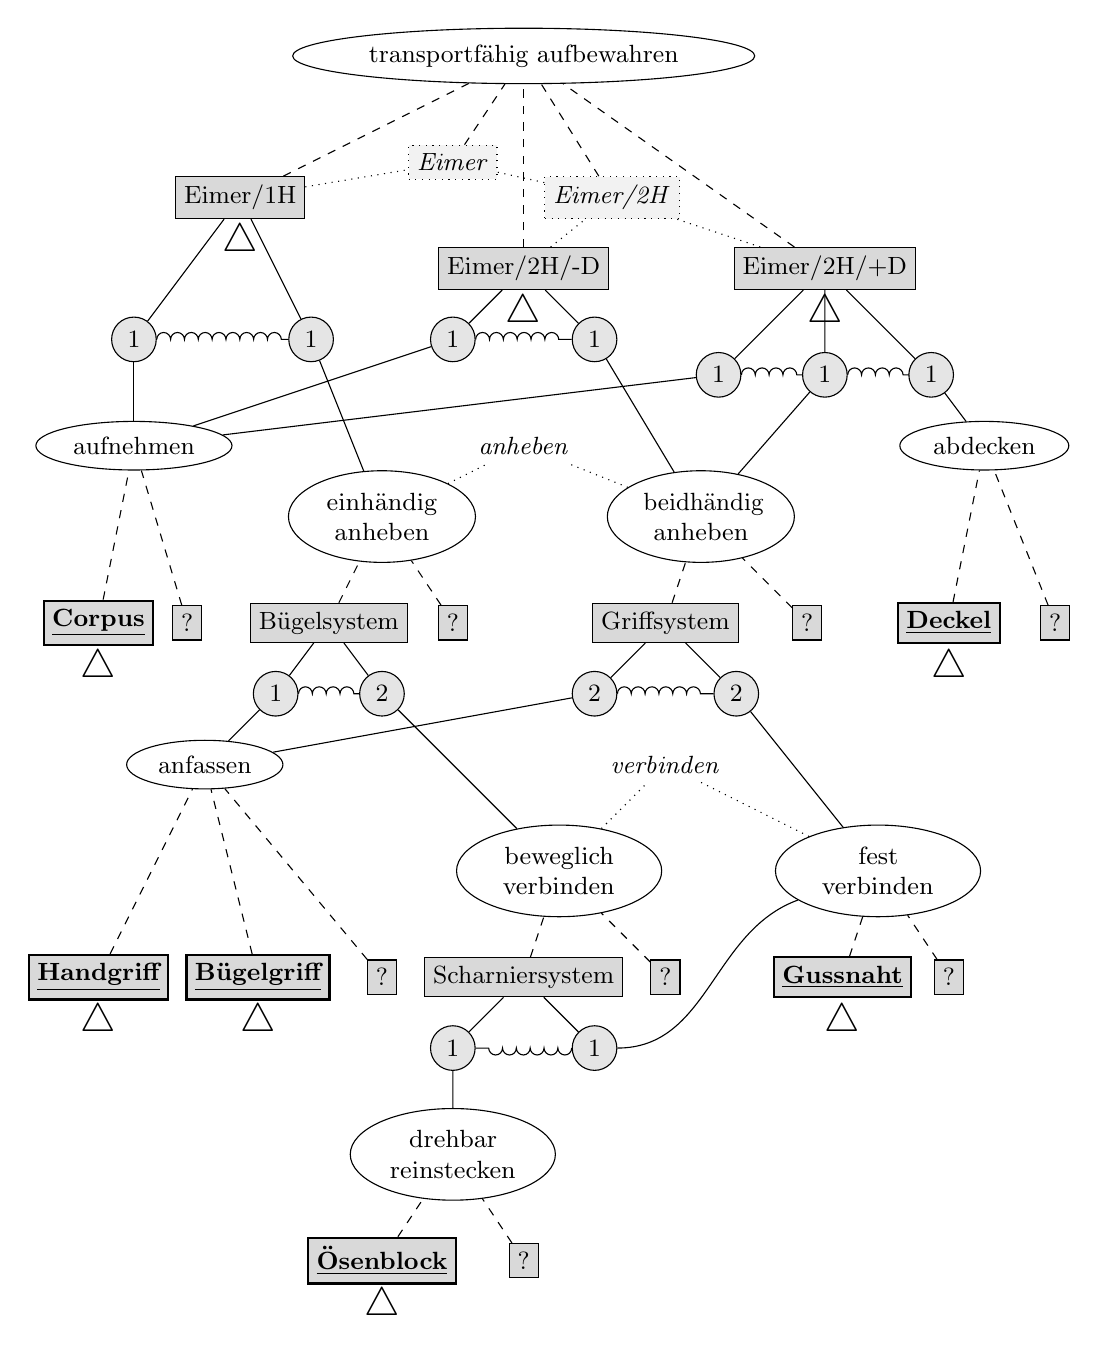
\begin{tikzpicture}[scale=0.9]
\small
\node[ellipse,draw] 
    (ps-15-01) at (6,17)
      {transportfähig aufbewahren};
 
 \node[rectangle,style={fill=gray!10,dotted},draw] 
    (pv-14-01) at (5,15.5) 
    {\textit{Eimer}};
      
 \node[rectangle,style={fill=gray!30},draw] 
    (pv-13-01) at (2,15) 
    {Eimer/1H}; 
    
 \node [] (pv-13-01-T) at (2,14.375) {\Large{$\triangle$}};
      
 \node[rectangle,style={fill=gray!10,dotted},draw] 
    (pv-13-02) at (7.25,15) 
    {\textit{Eimer/2H}};       

 \node[rectangle,style={fill=gray!30},draw] 
    (pv-12-01) at (6,14) 
    {Eimer/2H/-D}; 
 \node [] (pv-12-01-T) at (6,13.375) {\Large{$\triangle$}};
     
 \node[rectangle,style={fill=gray!30},draw] 
    (pv-12-02) at (10.25,14) 
    {Eimer/2H/+D}; 
 \node [] (pv-12-02-T) at (10.25,13.375) {\Large{$\triangle$}};
 
\node[circle,style={fill=gray!20},draw]  (sn-11-01) at (0.5,13) {1};
\node[circle,style={fill=gray!20},draw]  (sn-11-02) at (3,13) {1};
\node[circle,style={fill=gray!20},draw]  (sn-11-03) at (5,13) {1};
\node[circle,style={fill=gray!20},draw]  (sn-11-04) at (7,13) {1};
\node[circle,style={fill=gray!20},draw]  (sn-11-05) at (8.75,12.5) {1};
\node[circle,style={fill=gray!20},draw]  (sn-11-06) at (10.25,12.5) {1};
\node[circle,style={fill=gray!20},draw]  (sn-11-07) at (11.75,12.5) {1};

    
\node[ellipse,draw] 
    (ps-10-01) at (0.5,11.5)
      {aufnehmen};

\node[] 
    (ps-10-02) at (6,11.5)
      {\textit{anheben}};    

\node[ellipse,draw] 
    (ps-10-03) at (12.5,11.5)
      {abdecken};      
             
\node[ellipse,draw,text width=4.5em, text centered] 
    (ps-09-01) at (4,10.5)
      {einhändig anheben};
      
\node[ellipse,draw,text width=4.5em, text centered] 
    (ps-09-02) at (8.5,10.5)
      {beidhändig anheben};

\node[rectangle,style={fill=gray!30,thick},draw] 
    (pv-08-01) at (0,9) 
    {\textbf{\underline{Corpus}}};     
\node [] (pv-08-01-T) at (0,8.375) {\Large{$\triangle$}};
      
\node[rectangle,style={fill=gray!30},draw] 
    (pv-08-02) at (1.25,9) 
    {?};
    
\node[rectangle,style={fill=gray!30},draw] 
    (pv-08-03) at (8,9) 
    {Griffsystem};     
    
\node[rectangle,style={fill=gray!30},draw] 
    (pv-08-04) at (10,9) 
    {?};    
    
\node[rectangle,style={fill=gray!30},draw] 
    (pv-08-05) at (3.25,9) 
    {Bügelsystem};
    
\node[rectangle,style={fill=gray!30},draw] 
    (pv-08-06) at (5,9) 
    {?};
    
\node[rectangle,style={fill=gray!30,thick},draw] 
    (pv-08-07) at (12,9) 
    {\textbf{\underline{Deckel}}};     
\node [] (pv-08-07-T) at (12,8.375) {\Large{$\triangle$}};
    
\node[rectangle,style={fill=gray!30},draw] 
    (pv-08-08) at (13.5,9) 
    {?};
          
\node[circle,style={fill=gray!20},draw]  (sn-07-01) at (7,8) {2};
\node[circle,style={fill=gray!20},draw]  (sn-07-02) at (9,8) {2};
\node[circle,style={fill=gray!20},draw]  (sn-07-03) at (2.5,8) {1};
\node[circle,style={fill=gray!20},draw]  (sn-07-04) at (4,8) {2};

\node[ellipse,draw] 
    (ps-06-01) at (1.5,7)
    {anfassen};
 
\node[] 
    (ps-06-02) at (8,7)
    {\textit{verbinden}};
    
\node[ellipse,draw,text width=5em, text centered] 
    (ps-05-01) at (11,5.5)
    {fest verbinden};          

\node[ellipse,draw,text width=5em, text centered]
    (ps-05-02) at (6.5,5.5)
    {beweglich verbinden};       


\node[rectangle,style={fill=gray!30,thick},draw] 
    (pv-04-01) at (0,4) 
    {\textbf{\underline{Handgriff}}}; 
\node [] (pv-04-01-T) at (0,3.375) {\Large{$\triangle$}};

\node[rectangle,style={fill=gray!30,thick},draw] 
    (pv-04-02) at (2.25,4) 
    {\textbf{\underline{Bügelgriff}}}; 
\node [] (pv-04-02-T) at (2.25,3.375) {\Large{$\triangle$}};
           
\node[rectangle,style={fill=gray!30},draw] 
    (pv-04-03) at (4,4) 
    {?};           

\node[rectangle,style={fill=gray!30,thick},draw] 
    (pv-04-04) at (10.5,4) 
    {\textbf{\underline{Gussnaht}}};
\node [] (pv-04-04-T) at (10.5,3.375) {\Large{$\triangle$}};
 
\node[rectangle,style={fill=gray!30},draw] 
    (pv-04-05) at (12,4) 
    {?};  
    
\node[rectangle,style={fill=gray!30},draw] 
    (pv-04-06) at (6,4) 
    {Scharniersystem};

\node[rectangle,style={fill=gray!30},draw] 
    (pv-04-07) at (8,4) 
    {?};      

\node[circle,style={fill=gray!20},draw]  (sn-03-01) at (7,3) {1};
\node[circle,style={fill=gray!20},draw]  (sn-03-02) at (5,3) {1};
  
\node[ellipse,draw,text width=5em, text centered] 
    (ps-02-01) at (5,1.5)
    {drehbar reinstecken};   

\node[rectangle,style={fill=gray!30,thick},draw] 
    (pv-00-01) at (4,0) 
    {\textbf{\underline{Ösenblock}}};
 \node[] (pv-00-01-T) at (4,-0.635) {\Large{$\triangle$}};
 
\node[rectangle,style={fill=gray!30},draw] 
    (pv-00-02) at (6,0) 
    {?}; 



\foreach \from/\to in
  {pv-00-01/ps-02-01,pv-00-02/ps-02-01,
  pv-04-04/ps-05-01,pv-04-05/ps-05-01,
  pv-04-01/ps-06-01,pv-04-02/ps-06-01,pv-04-03/ps-06-01,
  pv-04-06/ps-05-02,pv-04-07/ps-05-02,
  pv-08-03/ps-09-02, pv-08-04/ps-09-02,
  pv-08-05/ps-09-01,pv-08-06/ps-09-01,
  pv-08-01/ps-10-01,pv-08-02/ps-10-01,
  pv-08-07/ps-10-03,pv-08-08/ps-10-03,
  pv-12-01/ps-15-01,pv-12-02/ps-15-01,pv-13-01/ps-15-01,pv-13-02/ps-15-01,
  pv-14-01/ps-15-01}
  \draw [dashed] (\from) -- (\to);
                   
\foreach \from/\to in
  {sn-03-01/pv-04-06,ps-02-01/sn-03-02,sn-03-02/pv-04-06,
  ps-06-01/sn-07-01,sn-07-01/pv-08-03,ps-05-01/sn-07-02,sn-07-02/pv-08-03,
  ps-06-01/sn-07-03,sn-07-03/pv-08-05,ps-05-02/sn-07-04,sn-07-04/pv-08-05,
  ps-10-01/sn-11-01,sn-11-01/pv-13-01,ps-09-01/sn-11-02,sn-11-02/pv-13-01,
  ps-10-01/sn-11-03,sn-11-03/pv-12-01,ps-09-02/sn-11-04,sn-11-04/pv-12-01,
  ps-10-01/sn-11-05,sn-11-05/pv-12-02,ps-09-02/sn-11-06,sn-11-06/pv-12-02,
  ps-10-03/sn-11-07,sn-11-07/pv-12-02}
  \draw (\from) -- (\to);
 
\foreach \from/\to in
  {pv-12-01/pv-13-02,pv-12-02/pv-13-02,pv-13-01/pv-14-01,pv-13-02/pv-14-01,
  ps-09-01/ps-10-02,ps-09-02/ps-10-02,ps-05-01/ps-06-02,ps-05-02/ps-06-02}
  \draw[dotted] (\from) -- (\to);

\foreach \from/\to in
  {sn-03-01/sn-03-02,sn-07-01/sn-07-02,sn-07-03/sn-07-04,
  sn-11-01/sn-11-02,sn-11-03/sn-11-04,sn-11-05/sn-11-06,sn-11-06/sn-11-07}
  \draw[snake=bumps] (\from) -- (\to);
                    
\draw (sn-03-01) to [out=0,in=200] (ps-05-01);

                         
 %\draw[help lines] (0,0) grid (15,18);              
             
\end{tikzpicture}


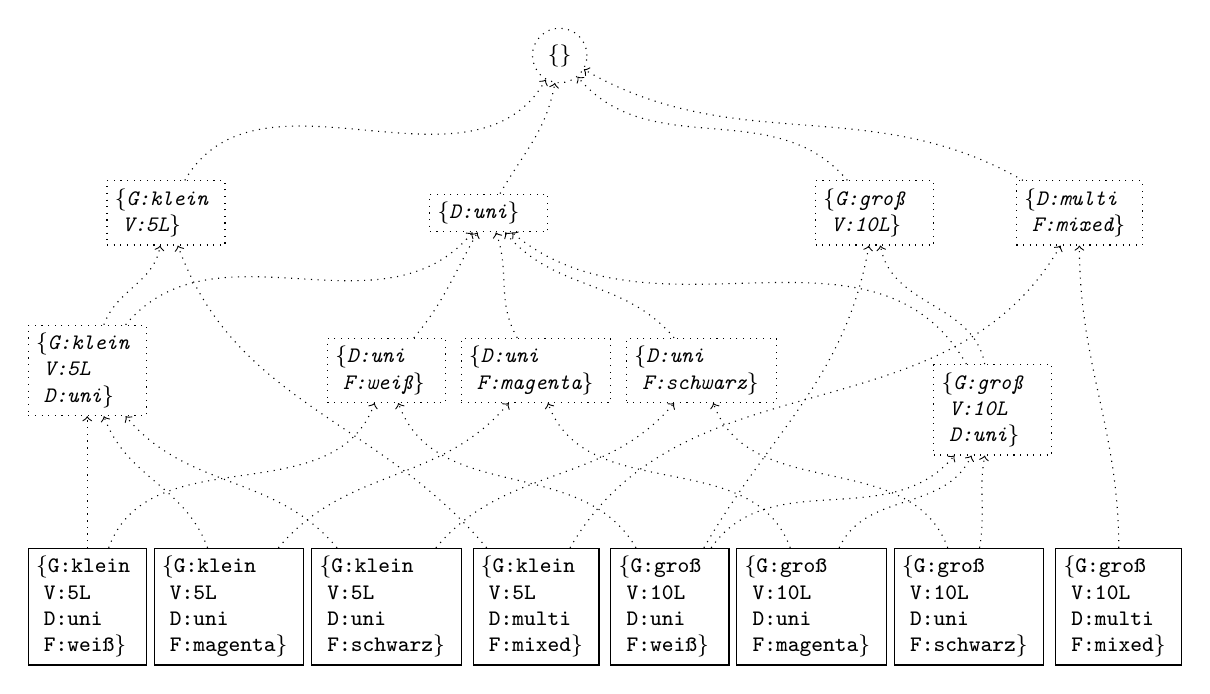
\begin{tikzpicture}
\label{SEKTAX}
\footnotesize

\node[rectangle,draw,text width=1.3cm] (c101) at (0,0)
{ \ttfamily{\{G:klein}\\
  \ttfamily{~V:5L}\\
  \ttfamily{~D:uni}\\
  \ttfamily{~F:weiß\}}
  };

\node[rectangle,draw,text width=1.7cm] (c102) at (1.8,0)
{ \ttfamily{\{G:klein}\\
  \ttfamily{~V:5L}\\
  \ttfamily{~D:uni}\\
  \ttfamily{~F:magenta\}}
  };

\node[rectangle,draw,text width=1.7cm] (c103) at (3.8,0)
{ \ttfamily{\{G:klein}\\
  \ttfamily{~V:5L}\\
  \ttfamily{~D:uni}\\
  \ttfamily{~F:schwarz\}}
  };

\node[rectangle,draw,text width=1.4cm] (c104) at (5.7,0)
{ \ttfamily{\{G:klein}\\
  \ttfamily{~V:5L}\\
  \ttfamily{~D:multi}\\
  \ttfamily{~F:mixed\}}
  };

\node[rectangle,draw,text width=1.3cm] (c105) at (7.4,0)
{ \ttfamily{\{G:groß}\\
  \ttfamily{~V:10L}\\
  \ttfamily{~D:uni}\\
  \ttfamily{~F:weiß\}}
  };

\node[rectangle,draw,text width=1.7cm] (c106) at (9.2,0)
{ \ttfamily{\{G:groß}\\
  \ttfamily{~V:10L}\\
  \ttfamily{~D:uni}\\
  \ttfamily{~F:magenta\}}
  };

\node[rectangle,draw,text width=1.7cm] (c107) at (11.2,0)
{ \ttfamily{\{G:groß}\\
  \ttfamily{~V:10L}\\
  \ttfamily{~D:uni}\\
  \ttfamily{~F:schwarz\}}
  };

\node[rectangle,draw,text width=1.4cm] (c108) at (13.1,0)
{ \ttfamily{\{G:groß}\\
  \ttfamily{~V:10L}\\
  \ttfamily{~D:multi}\\
  \ttfamily{~F:mixed\}}
  };
  


\node[rectangle,draw,text width=1.3cm,style={dotted}] (c201) at (0,3)
{ \textit{\ttfamily{\{G:klein}}\\
  \textit{\ttfamily{~V:5L}}\\
  \textit{\ttfamily{~D:uni\}}}
  };
  
 \node[rectangle,draw,text width=1.3cm,style={dotted}] (c202) at (1,5)
 { \textit{\ttfamily{\{G:klein}}\\
   \textit{\ttfamily{~V:5L\}}}
 };

 \node[rectangle,draw,text width=1.3cm,style={dotted}] (c203) at (3.8,3)
 { \textit{\ttfamily{\{D:uni}}\\
   \textit{\ttfamily{~F:weiß\}}}
 };


\node[rectangle,draw,text width=1.3cm,style={dotted}] (c204) at (5.1,5)
 { \textit{\ttfamily{\{D:uni\}}}
};

 \node[rectangle,draw,text width=1.7cm,style={dotted}] (c205) at (5.7,3)
 { \textit{\ttfamily{\{D:uni}}\\
   \textit{\ttfamily{~F:magenta\}}}
 };
 
  \node[rectangle,draw,text width=1.7cm,style={dotted}] (c206) at (7.8,3)
 { \textit{\ttfamily{\{D:uni}}\\
   \textit{\ttfamily{~F:schwarz\}}}
 };

 \node[rectangle,draw,text width=1.4cm,style={dotted}] (c207) at (12.6,5)
 { \textit{\ttfamily{\{D:multi}}\\
   \textit{\ttfamily{~F:mixed\}}}
 };

 

\node[rectangle,draw,text width=1.3cm,style={dotted}] (c208) at (11.5,2.5)
{ \textit{\ttfamily{\{G:groß}}\\
  \textit{\ttfamily{~V:10L}}\\
  \textit{\ttfamily{~D:uni\}}}
  };
  
\node[rectangle,draw,text width=1.3cm,style={dotted}] (c209) at (10,5)
{ \textit{\ttfamily{\{G:groß}}\\
  \textit{\ttfamily{~V:10L\}}}
  };

\node[circle,draw,style={dotted}] (c301) at (6,7)
{ \textit{\ttfamily{\{\}}}
  };
%evoked concept of level 2
%evoking c201
\draw[->,dotted] (c101) to [out=90,in=270] (c201);
\draw[->,dotted] (c102) to [out=110,in=290] (c201);
\draw[->,dotted] (c103) to [out=130,in=310] (c201);
%evoking c202
\draw[->,dotted] (c201) to [out=70,in=260] (c202);
\draw[->,dotted] (c104) to [out=130,in=290] (c202);

%evoking c203
\draw[->,dotted] (c101) to [out=70,in=250] (c203);
\draw[->,dotted] (c105) to [out=120,in=290] (c203);
%evoking c204
\draw[->,dotted] (c201) to [out=50,in=230] (c204);
\draw[->,dotted] (c203) to [out=50,in=240] (c204);

\draw[->,dotted] (c205) to [out=120,in=290] (c204);
\draw[->,dotted] (c206) to [out=130,in=310] (c204);
\draw[->,dotted] (c208) to [out=120,in=320] (c204);
%evoking c205
\draw[->,dotted] (c102) to [out=50,in=230] (c205);
\draw[->,dotted] (c106) to [out=110,in=290] (c205);
%evoking 206
\draw[->,dotted] (c103) to [out=50,in=230] (c206);
\draw[->,dotted] (c107) to [out=110,in=290] (c206);
%evoking 207
\draw[->,dotted] (c104) to [out=60,in=240] (c207);
\draw[->,dotted] (c108) to [out=90,in=270] (c207);
%evoking 208
\draw[->,dotted] (c105) to [out=55,in=230] (c208);
\draw[->,dotted] (c106) to [out=65,in=245] (c208);
\draw[->,dotted] (c107) to [out=80,in=260] (c208);


%evoking 209
\draw[->,dotted] (c105) to [out=60,in=260] (c209);
\draw[->,dotted] (c208) to [out=100,in=280] (c209);

%evoking 301
\draw[->,dotted] (c202) to [out=60,in=240] (c301);
\draw[->,dotted] (c204) to [out=60,in=260] (c301);
\draw[->,dotted] (c207) to [out=150,in=330] (c301);
\draw[->,dotted] (c209) to [out=130,in=310] (c301);
\end{tikzpicture}


\end{document}
